\documentclass{beamer}
\usetheme{metropolis}
\usepackage{listings}
\usepackage{graphicx}
\usepackage{standalone}
\usepackage{tikz}
\usepackage{tabu}
\usepackage{tikz}
\usepackage{verbatim}
\usepackage{tcolorbox}
\usepackage{appendixnumberbeamer}
\usepackage{booktabs}
\usepackage[scale=2]{ccicons}
\usepackage{pgfplots}
\usepackage{xspace}
\usepackage{listings}
\usepackage{graphicx}
\usepgfplotslibrary{dateplot}
\usetikzlibrary{shapes,snakes}

\setbeamertemplate{frame footer}{\insertsection\ // \insertsubsection}

\title{Security Managment of ECM Applications}
\subtitle{Fachpraktikum Information Systems}
\author{Christoph Kleine, Tim Zwietasch, Constantin Weißer}
\date{\today}

\begin{document}



\lstdefinestyle{customc}{
  belowcaptionskip=1\baselineskip,
  breaklines=true,
  frame=L,
  xleftmargin=\parindent,
  language=java,
  showstringspaces=false,
  basicstyle=\footnotesize\ttfamily,
  keywordstyle=\bfseries\color{green!40!black},
  commentstyle=\itshape\color{purple!40!black},
  identifierstyle=\color{blue},
  stringstyle=\color{orange},
}

\lstdefinestyle{customasm}{
  belowcaptionskip=1\baselineskip,
  frame=L,
  xleftmargin=\parindent,
  language=[x86masm]Assembler,
  basicstyle=\footnotesize\ttfamily,
  commentstyle=\itshape\color{purple!40!black},
}

\lstset{style=customc}



\frame{\titlepage}

\section{Introduction}
\subsection{Idea}
\begin{frame}
	\frametitle{Motivation}
	\begin{tcolorbox}[title=Overall Goal]
		Create an ECM portal for companies that do not want to host
		their data with one of the big providers. The focus is on
		usability and user-friendliness while maintaining security.
	\end{tcolorbox}

	\begin{itemize}
		\item Many companies prefer domestic small solutions
		\item Keep advantages of cloud solutions
		\item IBM's commercial portal as a model
	\end{itemize}
\end{frame}

\begin{frame}
	\frametitle{Motivation}
	\begin{tcolorbox}[title=Our Goal]
		Develop the user, groups and role management for this ECM portal
		based on open-source software.
	\end{tcolorbox}
	\begin{itemize}
		\item Easily extensible web application
		\item Usability
		\item Free and Open-Source Software (FOSS)
	\end{itemize}
\end{frame}

\subsection{FOSS}
\begin{frame}
	\frametitle{Open Source Software}
	\begin{tcolorbox}[title=Why use FOSS components?]
		\begin{itemize}
			\item no licensing costs
			\item[$\rightarrow$] good for scalability
			\item adaptivity and flexibility
			\item easier to find developers with expertise
			\item may perform code reviews (security)
		\end{itemize}
	\end{tcolorbox}
\end{frame}

\section{Security Model}
\subsection{Structure}
\begin{frame}
	\frametitle{Security Model}
	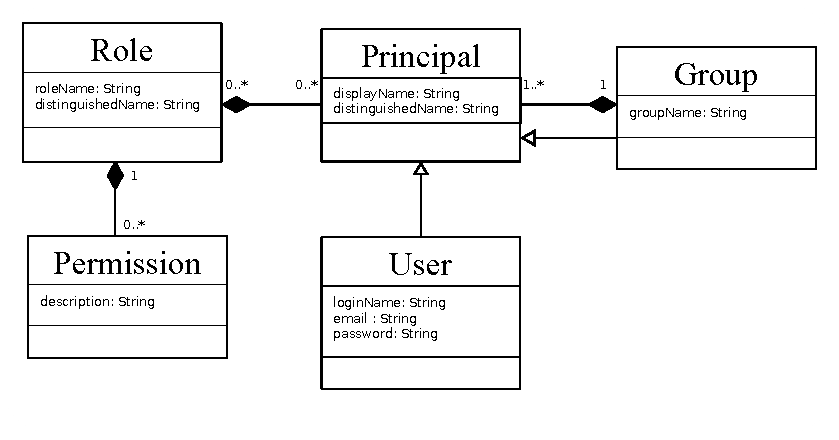
\includegraphics[width=\textwidth]{klassendiagramm.pdf}
\end{frame}

\section{Architecture}
\subsection{Overview}
\begin{frame}<1,2>[label=archgraph]
	\only<1,2>{%
		\frametitle{Architecture — Overview}
	}
	\only<3>{%
		\frametitle{Architecture — LDAP-Server}
	}
	\only<4>{%
		\frametitle{Architecture — Java middle layer}
	}
	\only<5>{%
		\frametitle{Architecture — Web-Application}
	}
	\begin{columns}[T]
		\begin{column}{0.48\textwidth}
			\begin{tikzpicture}
				\tikzset{every rectangle node/.style={draw, rectangle, color=gray}}
				\only<5>{%
					\tikzset{every rectangle node/.style={draw, rectangle, color=red}}
				}
				\node (frontend) at (0, 3) {Web-Application};
				\tikzset{every rectangle node/.style={draw, rectangle, color=gray}}
				\only<4>{%
					\tikzset{every rectangle node/.style={draw, rectangle, color=red}}
				}
				\node (middleend) at (0, 0) {Java middle layer};
				\tikzset{every rectangle node/.style={draw, rectangle, color=gray}}
				\only<3>{%
					\tikzset{every rectangle node/.style={draw, rectangle, color=red}}
				}
				\node (ldap) at (0, -3) {LDAP Server};

				\draw[<->] (frontend) to[] (middleend);
				\draw[<->] (middleend) to[] (ldap);
			\end{tikzpicture}
		\end{column}
		\begin{column}{0.48\textwidth}
			\only<2>{%
				\begin{itemize}
					\item Web-Application as user interface
					\item Java middle layer as intermediate program logic
					\item LDAP-Server as persistent storage
				\end{itemize}
			}
			\only<3>{%
				\begin{itemize}
					\item LDAP = ``Lightweight Directory Access Protocol''
					\item Persistence back-end (database)
					\item Authentication, querying and modification of data
					\item Data: users, groups, roles
					\item Roles are special groups
				\end{itemize}
			}
			\only<4>{%
				\begin{itemize}
					\item Connects front- with back-end
					\item REST interface
					\item Connects with LDAP-Server
					\item Accepts requests, executes, provides response
					\item Stateless
				\end{itemize}
			}
			\only<5>{%
				\begin{itemize}
					\item Based on Angular 2
					\item Makes REST calls to middle layer
					\item Displays data, responses, handles user interaction
					\item Attempt: minimize data transfer
				\end{itemize}
			}
		\end{column}
	\end{columns}
\end{frame}

\subsection{LDAP-Server}
\againframe<3>{archgraph}

\begin{frame}[fragile]
	\frametitle{LDAP Server Structure}
	\lstset{%
		basicstyle=\tiny
	}
	\begin{lstlisting}
SCCM: {
	bindusr : {...},
	customer: {
		groups: [
			...
		],
		users: [
			caseadmin: {
				cn: caseadmin,
				objectclass: inetOrgPerson,
				objectclass: organizationalPerson,
				objectclass: person,
				objectclass: top,
				sn: caseadmin,
				displayname: "Case Administrator",
				uid: caseadmin,
				userpassword: ***,
				...
			},
			domainadmin: {...},
			...
		]
	}
}
	\end{lstlisting}
\end{frame}

\subsection{Middle Layer}
\againframe<4>{archgraph}

\begin{frame}
	\frametitle{Middle Layer}
	\begin{itemize}
		\item Written in Java
		\item Uses Jersey to provide REST interface
		\item Shallow model of data
			\begin{itemize}
				\item User
				\item Group
				\item Role
			\end{itemize}
		\item Actions to manipulate data and query data
		\item \dots\ are passed through to back-end using LDAP requests
		\item \textbf{Authentication}: protects back-end from
			unauthorized access
	\end{itemize}
\end{frame}

\begin{frame}[fragile]
	\frametitle{Example Request}
	%TODO: nach java middlekack: "Beispiel Request"
	\textbf{Example Query:} Get X users at position Y
	\begin{itemize}
	 \item Receive filtered enumeration from LDAP containing users in the specified range Y to X
	 \item Build list of users
	 \item Send Response to Application Layer
	\end{itemize}
\begin{lstlisting}[frame=single]
public NamingEnumeration<SearchResult> search(
            String base,
            String filter,
            Object[] filterArgs,
            int limit ) throws NamingException
\end{lstlisting}
\end{frame}

\subsection{Frontend}
\againframe<5>{archgraph}

\begin{frame}
	\frametitle{Angular 2 \& Typescript}
	\begin{itemize}
		\item Javascript framework for web applications
		\item True object oriented web development
		\item Typescript syntax similar to Java 8
		\item Performance, scalability, cross-platform
		\item Google engineering director Brad Green (March, 2016):\\
		\emph{1.3 million developers use AngularJS and over 300 thousand are already using the soon to be released Angular 2}
	\end{itemize}
\end{frame}

\begin{frame}[fragile]
	\frametitle{Angular 2 Application}
	\begin{itemize}
		\item Tree of loosely coupled components
	\end{itemize}
	\begin{lstlisting}[frame=single]
<tabs>
  <tab title="Welcome">...</tab>
  <tab title="Security Configuration"> 
    <menu> 
      <item title="Users, Groups and Roles">
        <item title="Users">
          <users></users>
        </item>
        <item title="Groups">
          <groups></groups>
        </item>
...
	\end{lstlisting}
\end{frame}

\begin{frame}[fragile]
	\frametitle{Angular 2 Component}
	\lstset{%
		basicstyle=\tiny
	}
	\begin{lstlisting}[frame=single]
import { Group } from './group';
import { GroupsService } from './groups.service';
...
import { LDAPHttpService } from './../../shared/services/ldap-http.service'
@Component({
selector: 'groups',
templateUrl: './../templates/groups.tpl.html',
directives: [MODAL_DIRECTIVES, TABLE_DIRECTIVES, MENUBAR_DIRECTIVES],
providers: []
moduleId: module.id
})
export class Groups {
  public groups: Array<Group> = new Array<Group>();
  constructor(
    private ldapHttpService: LDAPHttpService,
    private groupsService: GroupsService, ...
  ){}
  // Showcase
  @Input('data') data: string = "default value";
  @Output() selected: EventEmitter<any> = new EventEmitter();
  ...
}
// Inside another template
<groups [data]="'new value'" (selected)="doSomething()">...</groups>
	\end{lstlisting}
\end{frame}

\section{Demonstration}

\section{Questions?}

\end{document}
